\documentclass{standalone}
\usepackage{tikz}
\usetikzlibrary{patterns, positioning}
\usepackage[sfdefault]{ClearSans} %% option 'sfdefault' activates Clear Sans as the default text font
\usepackage[T1]{fontenc}

\begin{document}
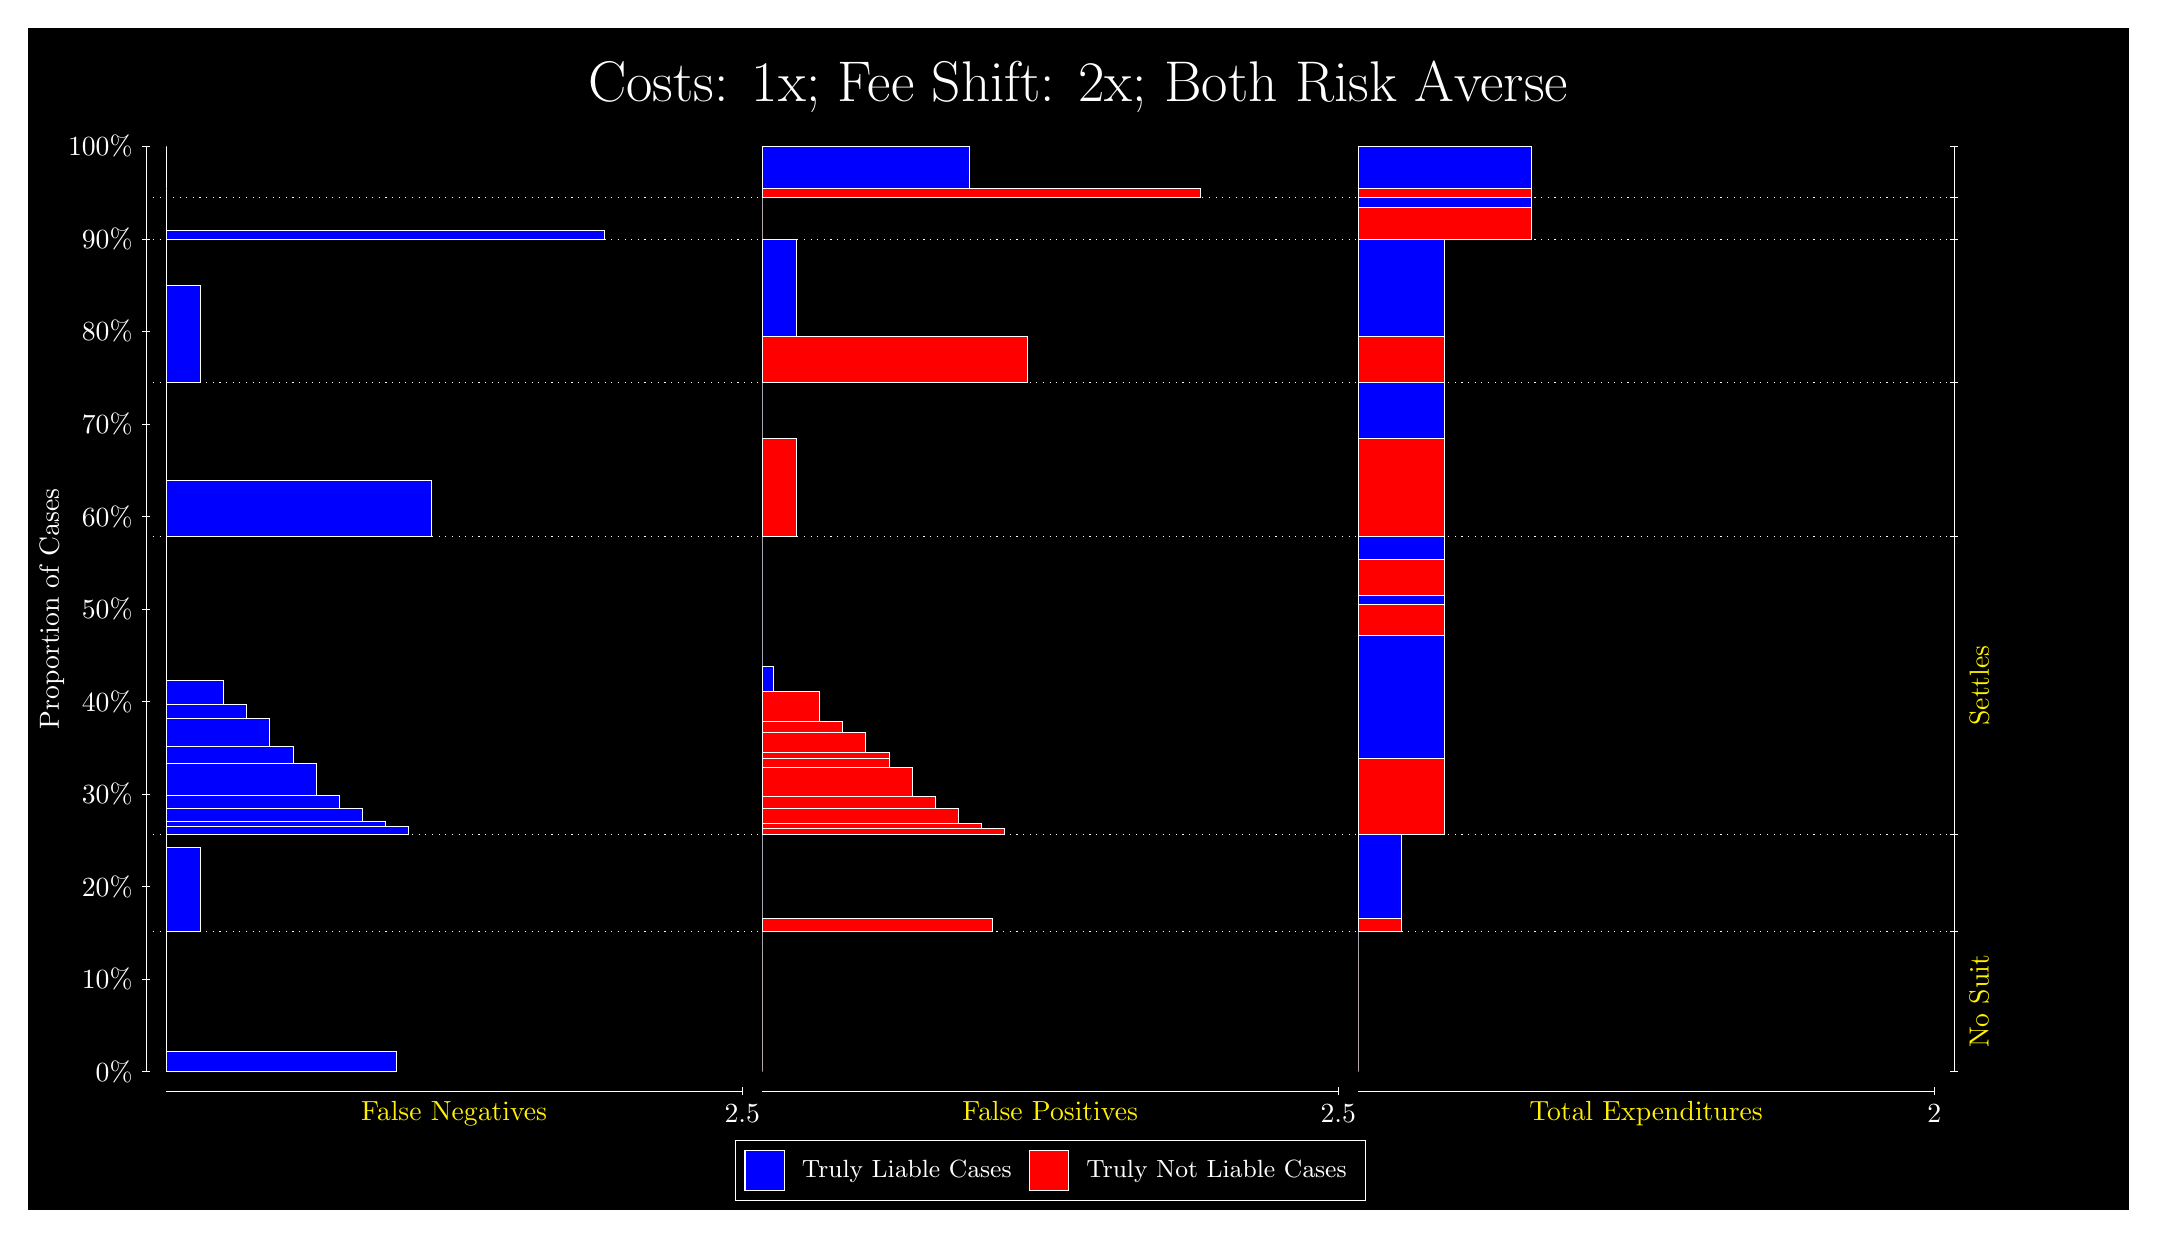
\begin{tikzpicture}
\draw[fill=black] (0,0) rectangle (26.667,15);
\draw[text=white] (0,13.5) rectangle (26.667,15) node[midway] {\huge Costs: 1x; Fee Shift: 2x; Both Risk Averse};
\draw[white, very thin] (1.5,1.75) -- (1.5,13.5);
\node[rotate=90, text=white, anchor=center] at (0.3, 7.625) {Proportion of Cases};
\draw[white, very thin] (1.45,1.75) -- (1.55,1.75);
\node[text=white, anchor=east] at (1.45, 1.75) {0\%};
\draw[white, very thin] (1.45,2.925) -- (1.55,2.925);
\node[text=white, anchor=east] at (1.45, 2.925) {10\%};
\draw[white, very thin] (1.45,4.1) -- (1.55,4.1);
\node[text=white, anchor=east] at (1.45, 4.1) {20\%};
\draw[white, very thin] (1.45,5.275) -- (1.55,5.275);
\node[text=white, anchor=east] at (1.45, 5.275) {30\%};
\draw[white, very thin] (1.45,6.45) -- (1.55,6.45);
\node[text=white, anchor=east] at (1.45, 6.45) {40\%};
\draw[white, very thin] (1.45,7.625) -- (1.55,7.625);
\node[text=white, anchor=east] at (1.45, 7.625) {50\%};
\draw[white, very thin] (1.45,8.8) -- (1.55,8.8);
\node[text=white, anchor=east] at (1.45, 8.8) {60\%};
\draw[white, very thin] (1.45,9.975) -- (1.55,9.975);
\node[text=white, anchor=east] at (1.45, 9.975) {70\%};
\draw[white, very thin] (1.45,11.15) -- (1.55,11.15);
\node[text=white, anchor=east] at (1.45, 11.15) {80\%};
\draw[white, very thin] (1.45,12.325) -- (1.55,12.325);
\node[text=white, anchor=east] at (1.45, 12.325) {90\%};
\draw[white, very thin] (1.45,13.5) -- (1.55,13.5);
\node[text=white, anchor=east] at (1.45, 13.5) {100\%};

\draw[white, very thin] (24.457,1.75) -- (24.457,13.5);
\draw[white, very thin] (24.407,1.75) -- (24.507,1.75);
\node[anchor=west] at (24.407, 1.75) {};
\draw[white, very thin] (24.407,3.5311) -- (24.507,3.5311);
\node[anchor=west] at (24.407, 3.5311) {};
\draw[white, very thin] (24.407,4.7575) -- (24.507,4.7575);
\node[anchor=west] at (24.407, 4.7575) {};
\draw[white, very thin] (24.407,8.5448) -- (24.507,8.5448);
\node[anchor=west] at (24.407, 8.5448) {};
\draw[white, very thin] (24.407,10.506) -- (24.507,10.506);
\node[anchor=west] at (24.407, 10.506) {};
\draw[white, very thin] (24.407,12.314) -- (24.507,12.314);
\node[anchor=west] at (24.407, 12.314) {};
\draw[white, very thin] (24.407,12.849) -- (24.507,12.849);
\node[anchor=west] at (24.407, 12.849) {};
\draw[white, very thin] (24.407,13.5) -- (24.507,13.5);
\node[anchor=west] at (24.407, 13.5) {};

\draw[white, very thin, fill=blue] (1.75,1.75) rectangle (4.6775,2.0134);
\draw[white, very thin, fill=red] (1.75,2.0134) rectangle (1.75,3.5311);
\draw[white, very thin, fill=blue] (1.75,3.5311) rectangle (2.1891,4.595);
\draw[white, very thin, fill=red] (1.75,4.595) rectangle (1.75,4.7575);
\draw[white, very thin, fill=blue] (1.75,4.7575) rectangle (4.8239,4.869);
\draw[white, very thin, fill=blue] (1.75,4.869) rectangle (4.5312,4.9293);
\draw[white, very thin, fill=blue] (1.75,4.9293) rectangle (4.2384,5.0936);
\draw[white, very thin, fill=blue] (1.75,5.0936) rectangle (3.9457,5.2534);
\draw[white, very thin, fill=blue] (1.75,5.2534) rectangle (3.6529,5.66);
\draw[white, very thin, fill=blue] (1.75,5.66) rectangle (3.3602,5.8829);
\draw[white, very thin, fill=blue] (1.75,5.8829) rectangle (3.0674,6.2335);
\draw[white, very thin, fill=blue] (1.75,6.2335) rectangle (2.7746,6.408);
\draw[white, very thin, fill=blue] (1.75,6.408) rectangle (2.4819,6.7204);
\draw[white, very thin, fill=red] (1.75,6.7204) rectangle (1.75,8.5448);
\draw[white, very thin, fill=blue] (1.75,8.5448) rectangle (5.1167,9.2557);
\draw[white, very thin, fill=red] (1.75,9.2557) rectangle (1.75,10.506);
\draw[white, very thin, fill=blue] (1.75,10.506) rectangle (2.1891,11.73);
\draw[white, very thin, fill=red] (1.75,11.73) rectangle (1.75,12.314);
\draw[white, very thin, fill=blue] (1.75,12.314) rectangle (7.3123,12.431);
\draw[white, very thin, fill=red] (1.75,12.431) rectangle (1.75,12.849);
\draw[white, very thin, fill=red] (1.75,12.849) rectangle (1.75,12.966);
\draw[white, very thin, fill=blue] (1.75,12.966) rectangle (1.75,13.5);
\draw[white, very thin, fill=red] (9.3189,1.75) rectangle (9.3189,3.2677);
\draw[white, very thin, fill=blue] (9.3189,3.2677) rectangle (9.3189,3.5311);
\draw[white, very thin, fill=red] (9.3189,3.5311) rectangle (12.246,3.6937);
\draw[white, very thin, fill=blue] (9.3189,3.6937) rectangle (9.3189,4.7575);
\draw[white, very thin, fill=red] (9.3189,4.7575) rectangle (12.393,4.8343);
\draw[white, very thin, fill=red] (9.3189,4.8343) rectangle (12.1,4.9049);
\draw[white, very thin, fill=red] (9.3189,4.9049) rectangle (11.807,5.0871);
\draw[white, very thin, fill=red] (9.3189,5.0871) rectangle (11.515,5.2473);
\draw[white, very thin, fill=red] (9.3189,5.2473) rectangle (11.222,5.6183);
\draw[white, very thin, fill=red] (9.3189,5.6183) rectangle (10.929,5.7342);
\draw[white, very thin, fill=red] (9.3189,5.7342) rectangle (10.929,5.7996);
\draw[white, very thin, fill=red] (9.3189,5.7996) rectangle (10.636,6.0582);
\draw[white, very thin, fill=red] (9.3189,6.0582) rectangle (10.344,6.1922);
\draw[white, very thin, fill=red] (9.3189,6.1922) rectangle (10.051,6.5819);
\draw[white, very thin, fill=blue] (9.3189,6.5819) rectangle (9.4652,6.8943);
\draw[white, very thin, fill=blue] (9.3189,6.8943) rectangle (9.3189,8.5448);
\draw[white, very thin, fill=red] (9.3189,8.5448) rectangle (9.758,9.7954);
\draw[white, very thin, fill=blue] (9.3189,9.7954) rectangle (9.3189,10.506);
\draw[white, very thin, fill=red] (9.3189,10.506) rectangle (12.686,11.091);
\draw[white, very thin, fill=blue] (9.3189,11.091) rectangle (9.758,12.314);
\draw[white, very thin, fill=red] (9.3189,12.314) rectangle (9.3189,12.732);
\draw[white, very thin, fill=blue] (9.3189,12.732) rectangle (9.3189,12.849);
\draw[white, very thin, fill=red] (9.3189,12.849) rectangle (14.881,12.966);
\draw[white, very thin, fill=blue] (9.3189,12.966) rectangle (11.954,13.5);
\draw[white, very thin, fill=red] (16.888,1.75) rectangle (16.888,3.2677);
\draw[white, very thin, fill=blue] (16.888,3.2677) rectangle (16.888,3.5311);
\draw[white, very thin, fill=red] (16.888,3.5311) rectangle (17.437,3.6937);
\draw[white, very thin, fill=blue] (16.888,3.6937) rectangle (17.437,4.7575);
\draw[white, very thin, fill=red] (16.888,4.7575) rectangle (17.986,5.7342);
\draw[white, very thin, fill=blue] (16.888,5.7342) rectangle (17.986,7.294);
\draw[white, very thin, fill=red] (16.888,7.294) rectangle (17.986,7.6838);
\draw[white, very thin, fill=blue] (16.888,7.6838) rectangle (17.986,7.7953);
\draw[white, very thin, fill=red] (16.888,7.7953) rectangle (17.986,8.2533);
\draw[white, very thin, fill=blue] (16.888,8.2533) rectangle (17.986,8.5448);
\draw[white, very thin, fill=red] (16.888,8.5448) rectangle (17.986,9.7954);
\draw[white, very thin, fill=blue] (16.888,9.7954) rectangle (17.986,10.506);
\draw[white, very thin, fill=red] (16.888,10.506) rectangle (17.986,11.091);
\draw[white, very thin, fill=blue] (16.888,11.091) rectangle (17.986,12.314);
\draw[white, very thin, fill=red] (16.888,12.314) rectangle (19.083,12.732);
\draw[white, very thin, fill=blue] (16.888,12.732) rectangle (19.083,12.849);
\draw[white, very thin, fill=red] (16.888,12.849) rectangle (19.083,12.966);
\draw[white, very thin, fill=blue] (16.888,12.966) rectangle (19.083,13.5);
\draw[white, dotted] (1.5,3.5311) -- (24.457,3.5311);
\draw[white, dotted] (1.5,4.7575) -- (24.457,4.7575);
\draw[white, dotted] (1.5,8.5448) -- (24.457,8.5448);
\draw[white, dotted] (1.5,10.506) -- (24.457,10.506);
\draw[white, dotted] (1.5,12.314) -- (24.457,12.314);
\draw[white, dotted] (1.5,12.849) -- (24.457,12.849);
\draw[white, very thin] (1.75,1.5) -- (9.0689,1.5);
\node[text=yellow, anchor=north] at (5.4094, 1.5) {False Negatives};
\draw[white, very thin] (9.0689,1.45) -- (9.0689,1.55);
\node[text=white, anchor=north] at (9.0689, 1.45) {2.5};

\draw[white, very thin] (9.3189,1.5) -- (16.638,1.5);
\node[text=yellow, anchor=north] at (12.978, 1.5) {False Positives};
\draw[white, very thin] (16.638,1.45) -- (16.638,1.55);
\node[text=white, anchor=north] at (16.638, 1.45) {2.5};

\draw[white, very thin] (16.888,1.5) -- (24.207,1.5);
\node[text=yellow, anchor=north] at (20.547, 1.5) {Total Expenditures};
\draw[white, very thin] (24.207,1.45) -- (24.207,1.55);
\node[text=white, anchor=north] at (24.207, 1.45) {2};

\node[text=yellow, centered, rotate=90] at (24.777, 2.6406) {No Suit};

\node[text=yellow, centered, rotate=90] at (24.777, 6.6512) {Settles};





\draw (12.978300999999998,1.5) node[draw=none] (baseCoordinate) {};
\begin{scope}[align=center]
        \matrix[scale=0.5, draw=white, below=0.5cm of baseCoordinate, nodes={draw}, column sep=0.1cm]{
            \node[rectangle, draw, minimum width=0.5cm, minimum height=0.5cm, fill=blue] {}; &
            \node[draw=none, font=\small, text=white] (B) {Truly Liable Cases}; &
            \node[rectangle, draw, minimum width=0.5cm, minimum height=0.5cm, fill=red] {}; &
            \node[draw=none, font=\small, text=white] (B) {Truly Not Liable Cases}; \\
            };
\end{scope}

\end{tikzpicture}
\end{document}